\section{函数-下}\label{004}

\begin{flushright}{\kaishu 無名, 天地之始; 有名, 萬物之母. 常無, 欲以觀其妙; 常有, 欲以觀其徼. \\- 苏辙 『老子解』}\end{flushright}

\begin{tcolorbox}[size=fbox, breakable, enhanced jigsaw, title={单射, 满射, 双射 (injection, surjection,
bijection)}]

一个函数 $f:X\rightarrow Y$ 若满足, 如果 $a\neq b$ 则
$f(a)\neq f(b)$ 对于任何属于 $X$ 的 $a$ 和 $b$,
那么它便是\textbf{单射}的 (injection, one-to-one)\footnote{One-to-one
  是更``纯正''英语的说法, 比较通俗, injection 是来自法语的舶来词,
  更具高级感; 后面的 onto 和 surjection 同.}.

一个函数 $f:X\rightarrow Y$ , 若它的值域 (range) 和陪域 (codomain)
一致, 即对于任意 $y\in Y$, 都存在至少一个 $x\in X$ 满足
$f(x)=y$\footnote{介绍一下符号语言: $\exists$ - 存在; $\forall$ -
  对于所有. 于是这句话可以这么表述:
  $\forall y\in Y, \exists x\in X \text{ s.t. } f(x)=y$ (s.t.=such that
  可以译为``使得''). 但是通常情况下,
  还是尽量避免符号语言而使用自然语言来描述.}, 那么它便是\textbf{满射}的
(surjection, onto).

一个同时单射又满射的函数是\textbf{双射}的 (bijection, one-to-one
correspondance).

还是以Captial这个函数为例子, 下面给出了单射, 满射,
双射三种情况分别的图示:

\begin{tcolorbox}[size=fbox, breakable, enhanced jigsaw]
\begin{center}
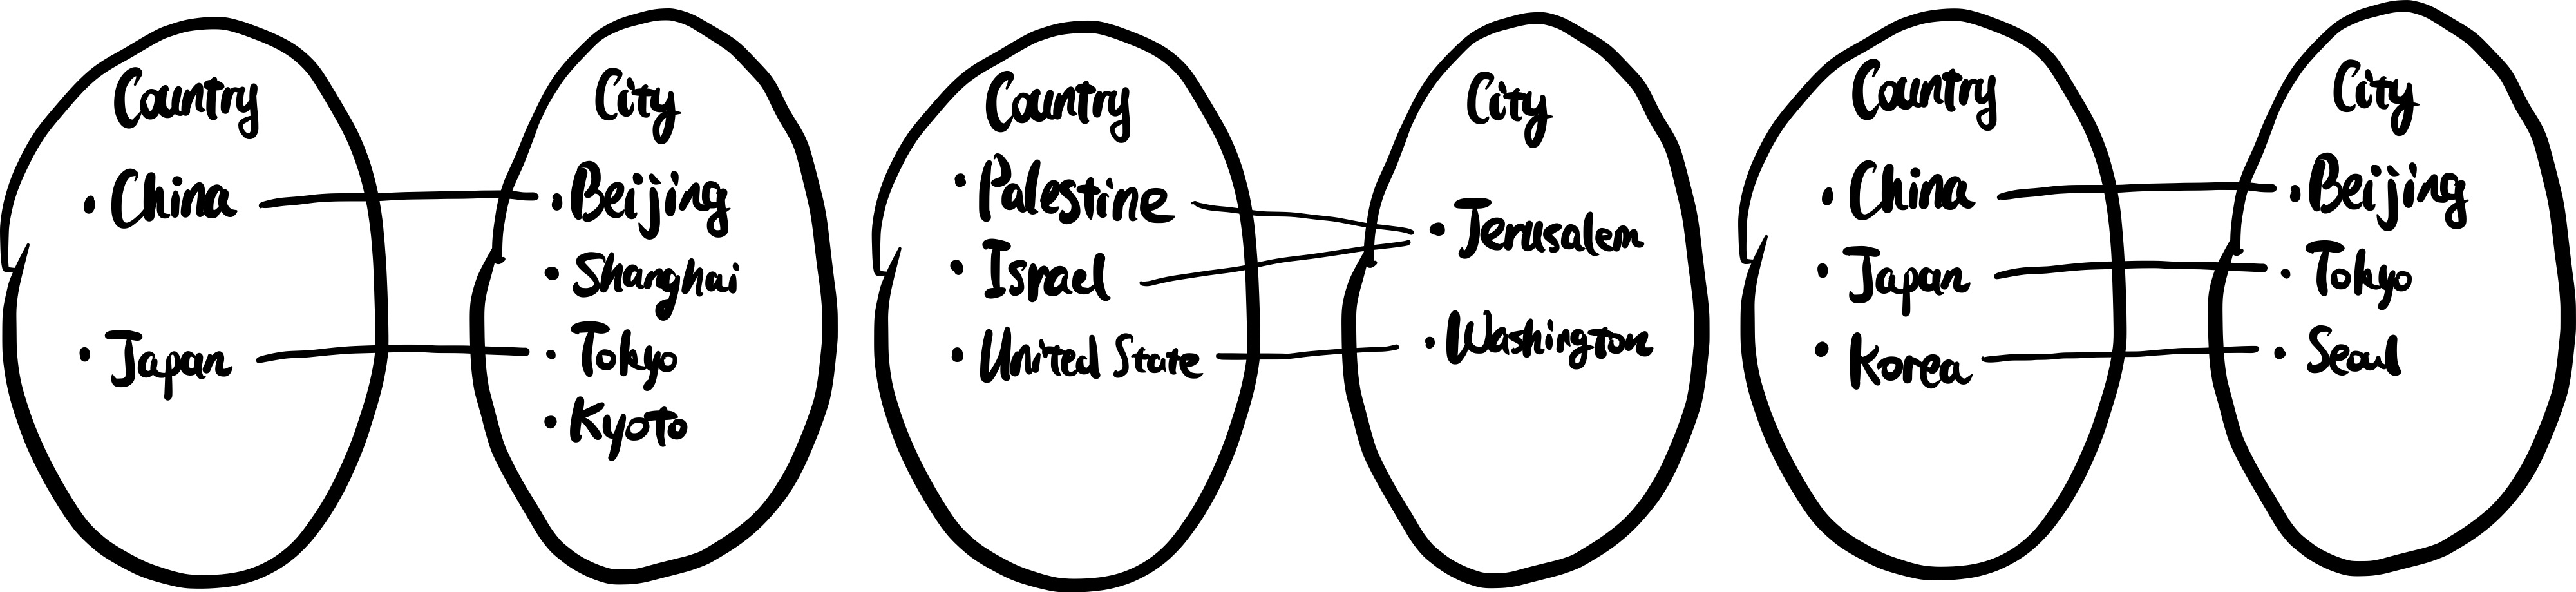
\includegraphics[width=0.9\textwidth]{img/image-20230302091706069.png}
\end{center}

\kaishu{\small 左: 单射但不满射; 中: 满射但不单射; 右: 双射.}
\end{tcolorbox}

\end{tcolorbox}

\begin{tcolorbox}[size=fbox, breakable, enhanced jigsaw, title={奇偶性 (parity 大嘘)}]

若一个函数满足 $f(-x)=-f(x)$, 即改变输入值 (自变量) 的正负号, 输出值
(因变量) 的正负号也改变, 这个函数便是\textbf{奇函数} (odd function).
图像上它是关于原点对称的.

若一个函数满足 $f(-x)=f(x)$, 即改变输入值 (自变量) 的正负号,
不影响输出值 (因变量) , 这个函数便是\textbf{偶函数} (even function).
图像上它是关于 $y$ 轴对称的.

当然, 奇函数和偶函数事实上是很特殊的两类函数,
更多的函数既不是奇函数又不是偶函数.

一些运算规律:

\begin{itemize}

\item
  奇函数 + 奇函数 = 奇函数\\{\kaishu 证明}: 假设存在两个奇函数 $f(x)$ 和
  $g(x)$, 令 $(f+g)(x) := f(x) + g(x)$, 即 $(f+g)(x)$
  这个函数是原本两函数之和. 根据奇函数的定义, $f(-x)=-f(x)$ 且
  $g(-x)=-g(x)$, 将两式相加得 $f(-x)+g(-x)=-f(x)-g(x)$, 即有
  $(f+x)(-x)=-(f+g)(x)$, 可见 $(f+g)(x)$ 是奇函数.
\item
  偶函数 + 偶函数 = 偶函数\\本条及接下来的证明与上一条类似, 可以当作练习.
\item
  奇函数 ×/÷ 奇函数 = 偶函数
\item
  偶函数 ×/÷ 偶函数 = 偶函数
\item
  奇函数 ×/÷ 偶函数 = 奇函数
\item
  偶函数 ×/÷ 奇函数 = 奇函数
\end{itemize}

\end{tcolorbox}

\begin{tcolorbox}[size=fbox, breakable, enhanced jigsaw, title={反函数 (inverse
function)}]

浅浅地非专业地叙述一下反函数. 设函数 $y=f(x)\ (x\in X)$ 的值域是
$Y$, 若存在一个函数 $g(y)$ 使得 $x= g(y)\ (y\in C)$, $g(x)$
便叫做 $f(x)$ 的\textbf{反函数} (inverse function), 可以记作
$x=f^{-1}(y)$, 它的定义域和值域分别是原函数的值域和定义域。

图像上, 反函数和原函数关于 $y=x$ 对称.

在求反函数时要特别注意反函数与原函数的定义域和值域. 例如 $y=f(x)=x^2$,
因为 $(\pm x)^2=y$, 反函数可能是 $x=f^{-1}(y)=\sqrt{y}$ 也可能是
$x=f^{-1}(y)=-\sqrt{y}$ , 但是不能是 $x=f^{-1}(y)=\pm\sqrt{y}$,
因为这样便不符合函数定义了, 一个输入值不可以有多个输出值,
或则说一个自变量不能对应多个因变量
(但是多个因变量对应一个自变量是允许的, 可以参考满射但不单射的图例).
这里反函数取正或负取决于原函数的定义域, 若 $y=f(x)=x^2, x\ge 0$, 则
$x=f^{-1}(y)=\sqrt{y}$; 若 $y=f(x)=x^2, x\le 0$, 则
$x=f^{-1}(y)=-\sqrt{y}$.

\end{tcolorbox}

\begin{tcolorbox}[size=fbox, breakable, enhanced jigsaw, title={隐函数 (implicit
function)}]

有的时候可能需要用函数来表达一个比较复杂的图像, 举一个简单一点的例子,
一个圆心位于原点的单位圆, 圆上任意一点到圆心距离都是 $1$, 于是有
$x^2+y^2=1$, 用前面学习的函数的形式表达这个关系, 有

$y=\begin{cases}\sqrt{1-x^2}\\-\sqrt{1-x^2}\end{cases}.$

这样似乎还没有起先的 $x^2+y^2=1$ 这个形式美观, 因此不妨还是用
$x^2+y^2-1=0$ 来表述单位圆上的 $x$ 与 $y$ 的关系. 类似这样,
利用一个【同时关于 $x$ 与 $y$ 的表达式 $F(x,y)=0$】来确定【 $y$
关于 $x$ 的函数】的表达式, 我们称之为\textbf{隐函数} (implicit
function); 为表区分, 前面介绍的类似 $y=f(x)$ 的函数,
称为\textbf{显函数} (explicit function).

\end{tcolorbox}

\begin{tcolorbox}[size=fbox, breakable, enhanced jigsaw, title={线性 (linearity)}]

这是一个很好的特性, 并不局限于函数, 仅对于函数来说的话,
若一个函数是线性的, 便有

$f(a+b)=f(a)+f(b),\ f(ax)=af(x).$

\end{tcolorbox}